% Created 2019-08-04 Sun 16:14
% Intended LaTeX compiler: pdflatex
\documentclass[11pt]{article}
\usepackage[utf8]{inputenc}
\usepackage[T1]{fontenc}
\usepackage{graphicx}
\usepackage{grffile}
\usepackage{longtable}
\usepackage{wrapfig}
\usepackage{rotating}
\usepackage[normalem]{ulem}
\usepackage{amsmath}
\usepackage{textcomp}
\usepackage{amssymb}
\usepackage{capt-of}
\usepackage{hyperref}
\usepackage[margin=1cm]{geometry}
\author{Wong Ding Feng}
\date{\today}
\title{Functional Programming: Real World Performance, Nix and Warp Server}
\hypersetup{
 pdfauthor={Wong Ding Feng},
 pdftitle={Functional Programming: Real World Performance, Nix and Warp Server},
 pdfkeywords={},
 pdfsubject={},
 pdfcreator={Emacs 26.2 (Org mode 9.2.2)}, 
 pdflang={English}}
\begin{document}

\maketitle
\tableofcontents

\section{Who am I? Introduction to myself}
\label{sec:orgea5e087}
\begin{itemize}
\item Follow me on github!
\url{https://github.com/TomatoCream}
\item Linux user for 5 years now
\begin{itemize}
\item Ubuntu
\item Proxmox
\item ArchLinux
\item Centos (server management)
\end{itemize}
\end{itemize}
\subsection{My interests}
\label{sec:org6d42dff}
\begin{itemize}
\item AI, ML
\item Functional programming and abstraction (what the hell is so good about this?)
\item philosophy
\begin{itemize}
\item occam's razor
\end{itemize}
\end{itemize}
\subsection{For whom is this talk for?}
\label{sec:org41cfc06}
\begin{itemize}
\item Linux users! Sorry windows users
\begin{itemize}
\item But not really (departs away from a unix way of doing things)
\end{itemize}
\item Show you what functional programming can do?
\begin{itemize}
\item purity?
\item referential transparency?
\end{itemize}
\item State management
\item DevOps
\item Images, Docker, VM, Clusters
\item I will give you a feel of \texttt{Nix} not the nitty gritty details
\end{itemize}
\section{The big problem, package manager wars!}
\label{sec:org0bd2b5c}
\begin{itemize}
\item What is the best package manager?
\item Has anyone ever used some sort of package management system?
\end{itemize}
\subsection{slant.co's opinions}
\label{sec:org415e91b}
\begin{center}
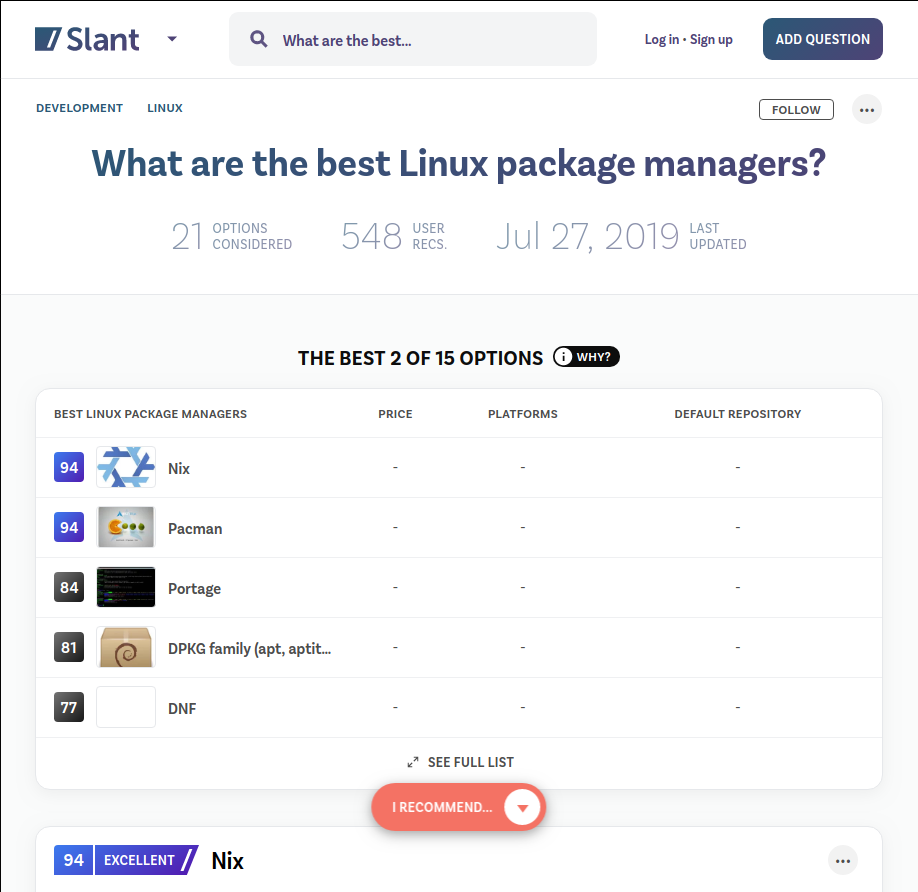
\includegraphics[width=.9\linewidth]{./images/screenshot-09.png}
\end{center}
\subsection{Some modern day package management systems}
\label{sec:orgd564c57}
\begin{center}
\begin{tabular}{ll}
Package manager & Distributions\\
\hline
apt, apt-get & Debian, Ubuntu\\
rpm, yum & Redhat, Centos\\
pacman & ArchLinux\\
brew & MacOS\\
\end{tabular}
\end{center}
\subsection{What about sub ecosystems?}
\label{sec:orgb99cead}
\begin{center}
\begin{tabular}{ll}
Package manager & ???\\
\hline
pip, virtualenv, pipenv & Python2,3(???)\\
npm, yarn & Nodejs\\
cabal, stack, hackage & Haskell :)\\
go? & go?\\
brew & MacOS\\
use-package, vim, fish, zsh & \ldots{}\\
\end{tabular}
\end{center}
\subsection{How to make a package manager?}
\label{sec:org0dbdef6}
\begin{itemize}
\item What are the basic parts that we need?
\end{itemize}
\subsection{How to make a package manager?}
\label{sec:orgcf364f7}
\begin{center}
\begin{tabular}{ll}
build dependencies & What do I need to build the program?\\
runtime dependencies & What \texttt{.so} shared objects do I need?\\
configurations & What in \texttt{/etc/...} config files\\
\end{tabular}
\end{center}
\begin{itemize}
\item essentially think of it as a graph, whenever we upgrade or install a package,
we are mutating a node on this graph to point to something else.
\end{itemize}
\subsubsection{real senario}
\label{sec:org5b2ff49}
\begin{verbatim}
pkgname=pacman
pkgver=5.1.0
_pkgver=1.0.0
pkgrel=2
pkgdesc="A library-based package manager with dependency support"
arch=('i686' 'x86_64')
url="http://www.archlinux.org/pacman/"
license=('GPL')
groups=('base' 'base-devel')
depends=('bash>=4.2.042-2' 'glibc>=2.17-2' 'libarchive>=3.1.2' 'curl>=7.39.0'
         'gpgme' 'archlinux-keyring' 'manjaro-keyring' 'pacman-mirrors>=4.1.0')
checkdepends=('python2' 'fakechroot')
makedepends=('asciidoc' 'pacman>=5.1')
optdepends=('haveged: for pacman-init.service')
provides=('pacman-contrib' 'pacman-init')
conflicts=('pacman-contrib' 'pacman-init')
replaces=('pacman-contrib' 'pacman-init')
backup=(etc/pacman.conf etc/makepkg.conf)
install=pacman.install
options=('strip' 'debug')
\end{verbatim}
\subsection{Problems with modern package management}
\label{sec:orgb21001e}
\url{https://wiki.debian.org/DontBreakDebian\#Don.27t\_make\_a\_FrankenDebian}
\begin{center}
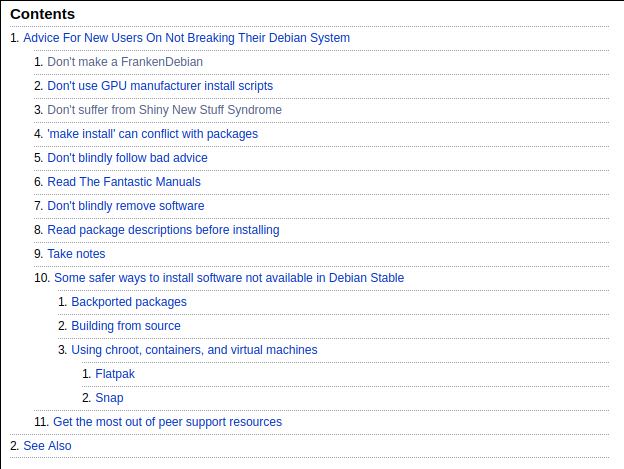
\includegraphics[width=.9\linewidth]{./images/screenshot-01.png}
\end{center}
\subsection{{\bfseries\sffamily TODO} Why imperative is bad? What is so imperative about installing packages?}
\label{sec:orgf1a56e9}
referential transparency
\subsection{Are you familiar with \texttt{DEPENDENCY HELL}?}
\label{sec:org6368281}
\begin{itemize}
\item \url{https://www.reddit.com/r/ProgrammerHumor/comments/75txp4/nodejs\_dependency\_hell\_visualized\_for\_the\_first/?utm\_source=share\&utm\_medium=web2x}
\item \url{https://github.com/vector-im/riot-web/network/dependencies}
\end{itemize}
\subsection{All types of "DEPENDENCY HELL"}
\label{sec:org474bce2}
\url{https://miro.medium.com/max/984/0*7ezJOtYUkI5zyqWU.png}
\begin{itemize}
\item \{ DLL, dependency, npm, cabal \} hell, different names for the same demon
\item conflicting dependency
\begin{itemize}
\item shared components like library links \texttt{cuda.7.so} vs \texttt{cuda.6.so}
\end{itemize}
\item multiple version side by side and roll backs
\item possible solutions
\begin{itemize}
\item set of stable packages like \texttt{Debian} or \texttt{haskell stack snapshots}
\end{itemize}
\end{itemize}
\subsection{Not Atomic 01}
\label{sec:org321eebf}
\begin{itemize}
\item kill upgrades half way
\begin{itemize}
\item packages left in a semi updated state
\item sometimes need to manually remove lock files
\end{itemize}
\end{itemize}
\begin{verbatim}
COMMAND   PID USER   FD   TYPE DEVICE SIZE/OFF   NODE NAME
dpkg    29329 root    3uW  REG    8,7        0 262367 /var/lib/dpkg/lock
\end{verbatim}
\subsection{Not Atomic 02}
\label{sec:org9ccc2bd}
\begin{itemize}
\item can be fixed but kinda troublesome.
\end{itemize}
\begin{center}
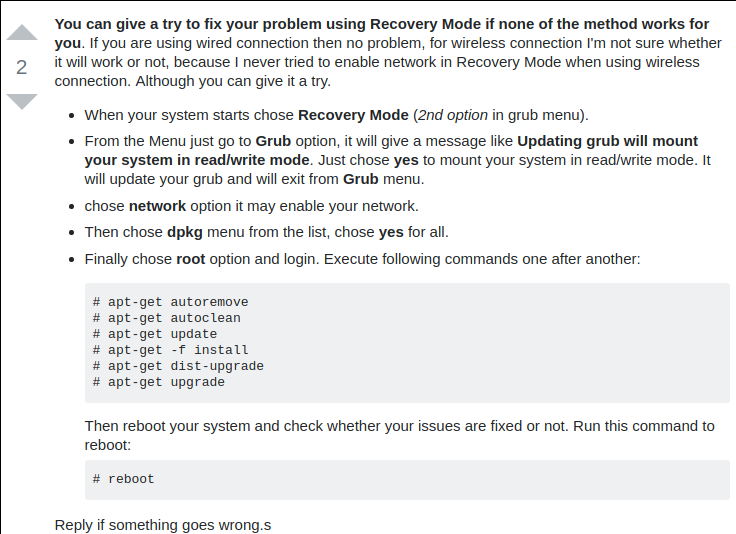
\includegraphics[width=.9\linewidth]{./images/screenshot-02.png}
\end{center}
\subsection{Whats bad about imperative summary?}
\label{sec:org9373028}
\begin{itemize}
\item No referential transparency
\begin{itemize}
\item cannot point to older versions of the same thing
\end{itemize}
\item Dependency hell
\begin{itemize}
\item conflicting dependencies
\end{itemize}
\item Not atomic upgrades
\begin{itemize}
\item unknown state if break half way
\end{itemize}
\end{itemize}
These problems are really similar to the problems with imperative languages!
like \texttt{JAVA} and people have already made solutions for them like how \texttt{Haskell}
does. We could learn a thing or two from them.
\section{What it should/could/would have been?}
\label{sec:orgdaded6e}
\begin{itemize}
\item Imagine now that we implemented all the things of a functional programming
language to create a functional package management system?
\item What can we do with this?
\end{itemize}
\subsection{GUIX vs Nix}
\label{sec:orga87bab6}
\begin{itemize}
\item \begin{center}

\includegraphics[width=.9\linewidth]{./images/screenshot-04.png}
\end{center}
\item \begin{center}
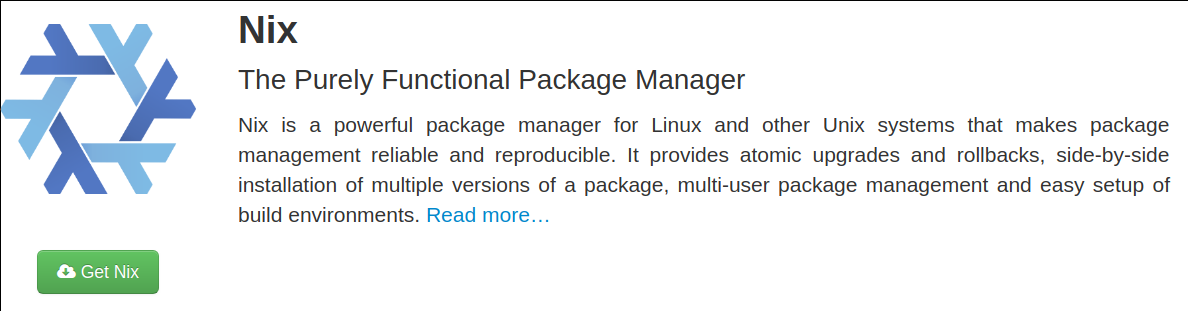
\includegraphics[width=.9\linewidth]{./images/screenshot-03.png}
\end{center}
\end{itemize}
\subsection{Introducing Nix Package Management}
\label{sec:org0bd899b}
\begin{itemize}
\item solves all of the problems above
\begin{itemize}
\item No referential transparency
\begin{itemize}
\item cannot point to older versions of the same thing
\end{itemize}
\item Dependency hell
\item Not atomic upgrades
\begin{itemize}
\item unknown state if break half way
\end{itemize}
\end{itemize}
\end{itemize}
\subsection{Main mechanism}
\label{sec:org3180dbb}
\begin{itemize}
\item referential transparency
\begin{itemize}
\item install everything in path \texttt{/nix/store/\{hash\}-name}
\item via \texttt{symlinking}
\end{itemize}
\end{itemize}
\subsection{What you get for free with this mechanism?}
\label{sec:org93e2cf7}
\begin{itemize}
\item no \texttt{sudo}
\item easy revert and roll back
\item select specific version
\item 2 different version can run at the same time
\item same \textbf{development} environment as the \textbf{runtime} environment!
\begin{itemize}
\item nix-shell
\end{itemize}
\end{itemize}
\subsubsection{no \texttt{sudo}, where is my \texttt{sudo}?}
\label{sec:orgf48159e}
\begin{itemize}
\item linux was developed as a \texttt{time sharing} system
\item many users were expected to share a single computer.
\item thus to manage conflicts, a \texttt{super user}, \texttt{root} was required to
install and manage packages
\begin{verbatim}
nix-env -iA nixos.figlet
\end{verbatim}
\end{itemize}
\subsubsection{easy revert, rollback}
\label{sec:orgf1596da}
\begin{verbatim}
figlet "I am here!"
\end{verbatim}
\begin{verbatim}
nix-env --rollback
\end{verbatim}
\begin{verbatim}
figlet "are you still here?"
\end{verbatim}
\subsubsection{Select specific version}
\label{sec:orgff973a3}
\begin{verbatim}
cd ~/projects/nix-config/
git checkout ??
nix-env -f ~/projects/nix-config/ -iA screenfetch
\end{verbatim}
screenfetch 2016 vs current
\subsubsection{Installing and running 2 version of same software}
\label{sec:org75b7672}
\begin{verbatim}
stack --version
su
stack --version
\end{verbatim}
\subsubsection{Same development environment and runtime environment}
\label{sec:orgbcda1af}
\begin{itemize}
\item I am not an electrical engineer or something but I program my
own keyboard. So I need some sort of firmware flasher. like
\texttt{dfuprogrammer} I dont need it on my system.
\end{itemize}
\begin{verbatim}
cd ~/projects/qmk_firmware/
make
dfuprogrammer
nix-shell
make
dfuprogrammer
\end{verbatim}
\subsection{Going all the way, NixOS}
\label{sec:org8030be9}
\begin{itemize}
\item whole system management via Nix and thus NixOS
\begin{itemize}
\item Version controlled operating system
\item show OS reboot
\item I wanted to show my generations so had been delaying removing
my older generations
\end{itemize}
\end{itemize}
\begin{verbatim}
df -h /
nix-collect-garbage --delete-older-than 10 --dry-run
\end{verbatim}
\subsubsection{NixOS}
\label{sec:org899d666}
\begin{itemize}
\item show \url{file:///home/df/nix-config/configuration.nix}
\item python package management \url{file:///home/df/nix-config/configuration.nix}
\item gnupg agent \url{file:///home/df/nix-config/configuration.nix}
\item ports \url{file:///home/df/nix-config/configuration.nix}
\begin{itemize}
\item I think it helps me get a state of all the ports in one place
\end{itemize}
\item users and security all in one place
\url{file:///home/df/nix-config/configuration.nix}
\begin{itemize}
\item authorisedkeys
\end{itemize}
\item postgresql can be packaged in \texttt{shell.nix}
\url{file:///home/df/nix-config/configuration.nix}
\begin{itemize}
\item separate project called \texttt{nixos-shell}
\url{https://github.com/chrisfarms/nixos-shell}
\end{itemize}
\item filesystems \url{file:///etc/nixos/hardware-configuration.nix}
\end{itemize}
\subsubsection{docker}
\label{sec:orgeaac453}
\url{https://nixos.wiki/wiki/Docker}
\begin{verbatim}
virtualisation.docker.enable = true;
users.users.<myuser>.extraGroups = [ "docker" ];
\end{verbatim}
\begin{verbatim}
nix-build '<nixpkgs>' -A dockerTools.examples.redis
docker load < result
\end{verbatim}
\url{https://github.com/NixOS/nixpkgs/blob/master/pkgs/build-support/docker/examples.nix}
\subsubsection{easy cd/dvd}
\label{sec:org6b8560b}
\begin{verbatim}
cd ~/projects/nixpkgs
nix-build -A config.system.build.isoImage -I nixos-config=modules/installer/cd-dvd/installation-cd-minimal.nix default.nix
\end{verbatim}
\subsubsection{easy vm}
\label{sec:orgbc432d5}
\begin{verbatim}
cd ./nixops
nixops create -d simple02 network.nix
nixops deploy -d simple02
\end{verbatim}
\begin{verbatim}
deployment.targetEnv = "ec2";
deployment.region = "eu-west-1";
\end{verbatim}
\section{How does nix actually work?}
\label{sec:org471266e}
\subsection{Nix expressions}
\label{sec:org8ad168e}
\begin{itemize}
\item functional expressions, not general purpose please do not program
things with it
\item comes with its own BNF grammar
\end{itemize}
\begin{center}
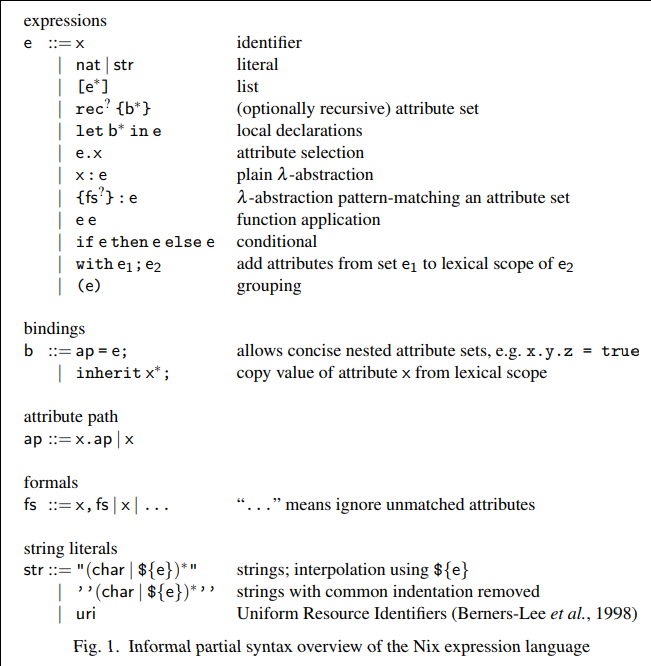
\includegraphics[width=.9\linewidth]{./images/screenshot-05.png}
\end{center}
\subsection{Language features}
\label{sec:org726a984}
\begin{itemize}
\item Nix expressions
\begin{itemize}
\item dynamically typed
\item lazy
\item pure
\end{itemize}
\end{itemize}
\subsection{The main point}
\label{sec:orgc8a7d80}
\begin{itemize}
\item Nix expressions are here to describe a graph of build actions
called \texttt{derivations}
\begin{itemize}
\item build script
\item set of environment variables
\item set of dependencies
\end{itemize}
\end{itemize}
\subsection{Example: Xmonad}
\label{sec:orgf84f6cb}
\begin{center}
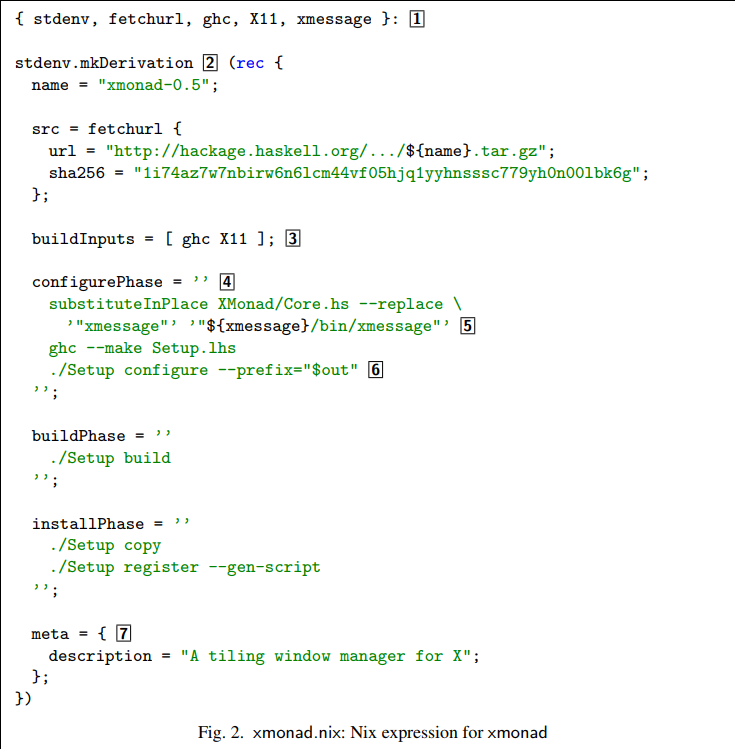
\includegraphics[width=.9\linewidth]{./images/screenshot-06.png}
\end{center}
\subsection{Example: Xmonad}
\label{sec:org094a504}
\begin{center}
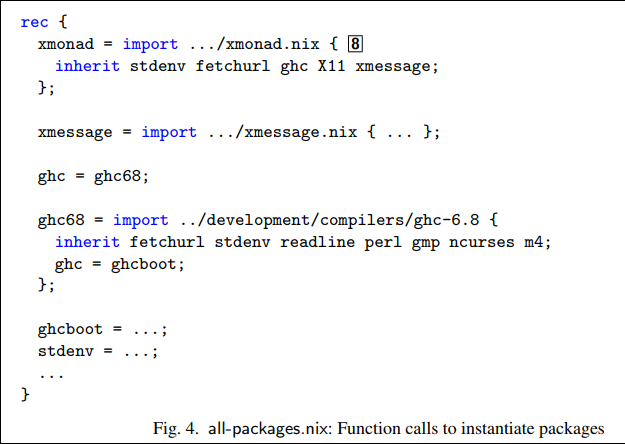
\includegraphics[width=.9\linewidth]{./images/screenshot-07.png}
\end{center}
\subsection{Main mechanism}
\label{sec:org67536a4}
\begin{center}
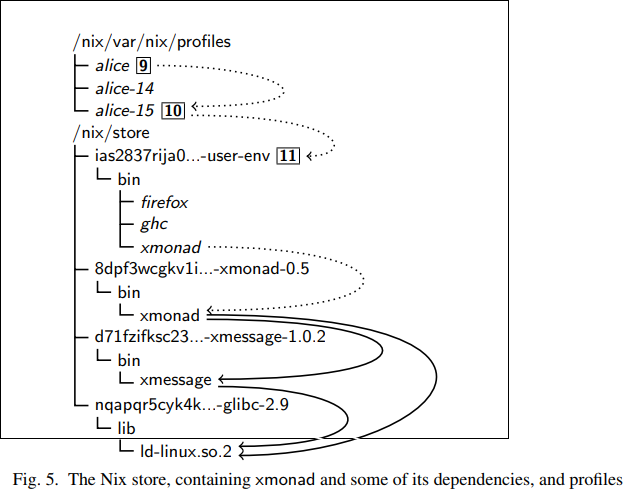
\includegraphics[width=.9\linewidth]{./images/screenshot-08.png}
\end{center}
\section{Nix as infrastructure (imagination)}
\label{sec:orgd8dbad9}
\begin{itemize}
\item how might one use nix in \texttt{JPMC's} infrastructure?
\end{itemize}
\subsection{Main componenets}
\label{sec:orga5af4ba}
\begin{itemize}
\item Hydra caching
\item Dependency management
\item Ease of use
\begin{itemize}
\item nix-shell
\end{itemize}
\item Security
\end{itemize}
\subsection{Caching build farm or cachix}
\label{sec:org39ace42}
\begin{center}
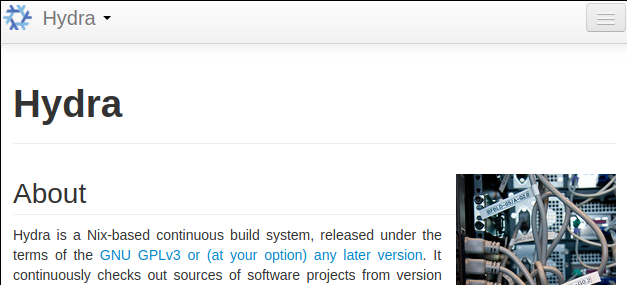
\includegraphics[width=.9\linewidth]{./images/screenshot-10.png}
\end{center}
\begin{center}

\includegraphics[width=.9\linewidth]{./images/screenshot-11.png}
\end{center}
\section{references}
\label{sec:org99d1ab5}
\begin{itemize}
\item\relax [HTML] Nix: A Safe and Policy-Free System for Software Deployment.
\begin{itemize}
\item E Dolstra, M De Jonge, E Visser - usenix.org
\item \url{https://nixos.org/\~eelco/pubs/nspfssd-lisa2004-final.pdf}
\end{itemize}
\item\relax [PDF] A Purely Functional Linux Distribution - NixOS
\begin{itemize}
\item E Dolstra
\item \url{https://nixos.org/\~eelco/pubs/nixos-jfp-final.pdf}
\end{itemize}
\item Hydra - NixOS
\begin{itemize}
\item \url{https://nixos.org/\~eelco/pubs/hydra-scp-submitted.pdf}
\end{itemize}
\end{itemize}
\end{document}
